\documentclass{article}
\usepackage{geometry}  
\usepackage{amsmath}  
\usepackage{graphicx} 
\usepackage{svg}
\usepackage[T1]{fontenc}
\usepackage{float}
\usepackage[utf8]{inputenc}

%----------------------------------------------------------------------------------------
%	REPORT INFORMATION
%----------------------------------------------------------------------------------------

\title{TRA - Techniki Realizacji Algorytmów Cyfrowego Przetwarzania Sygnałów  \\ Projekt - specyfikacja algorytmiczna \\} % Report title

\author{Anna \textsc{Dzieżyk}, indeks: 318506 \\ }% Author name(s), add additional authors like: '\& James \textsc{Smith}'

\date{\today} % Date of the report

%----------------------------------------------------------------------------------------

\begin{document}

\maketitle % Insert the title, author and date using the information specified above
\section{Wstęp}
Założeniem projektu jest porównnaie działania wzmacniacza klasy D, używanego często do zastosowań audio, gdzie 
rozdzielczość sygnału jest ważna, z różnymi stopniami wejściowymi. Badane stopnie wejściowe to będą: komparator oraz przetwornik sigma delta.
\begin{figure} [H]
    \centering
    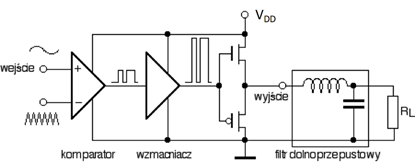
\includegraphics[scale=0.5]{D_calss_amp.png}
    \caption{Schemat blokowy całego typowego wzmacniacza klasy D}
\end{figure}
\section{Realizowane badane układy}
\subsection{Wzmacniacz klasy D z komparatorem jako stopniem wejściowym}
\begin{figure} [H]
	\begin{center}
			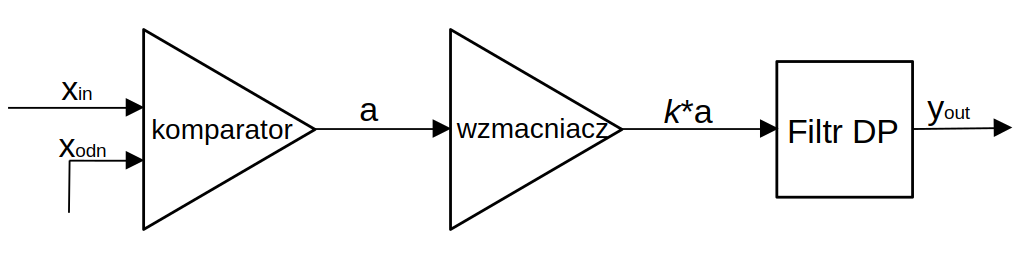
\includegraphics[width = \textwidth]{D_Class_amp_Comp_in.png}
            \caption{Schemat blokowy całego analizowanego wariantu wzmacniacza klasy D}
	\end{center}
\end{figure}

\begin{figure} [H]
	\begin{center}
			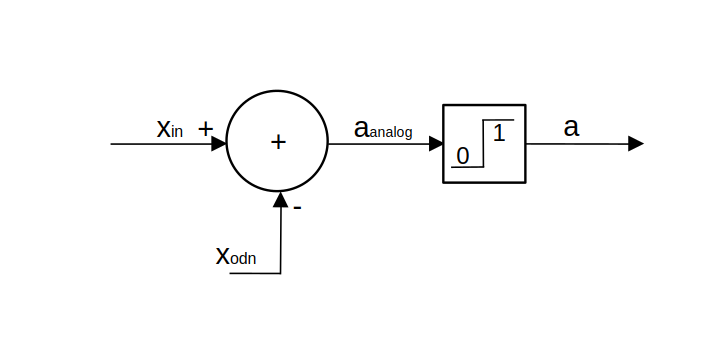
\includegraphics[scale = 0.5]{komparator_flowchart.png}
            \caption{Diagram przepływu sygnału w implementacji komparatora}
	\end{center}
\end{figure}

\subsection{Wzmacniacz klasy D z przetwornikiem Sigma-Delta od pierwszego do trzeciego rzędu jako stopniem wejściowym}
\begin{figure} [H]
	\begin{center}
			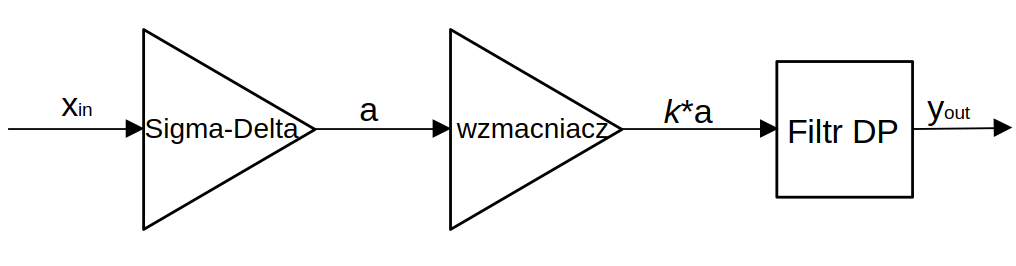
\includegraphics[width = \textwidth]{D_Class_amp_SD_in.png}
            \caption{Schemat blokowy całego analizowanego wariantu wzmacniacza klasy D}
	\end{center}
\end{figure}

\begin{figure} [H]
	\begin{center}
			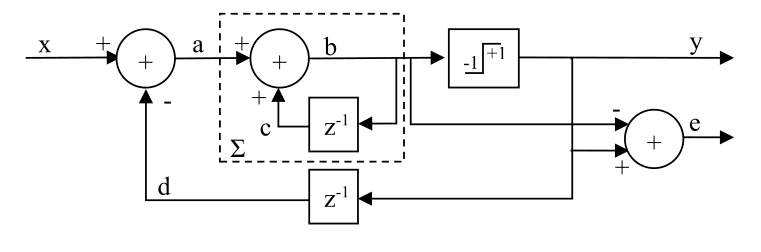
\includegraphics[width = \textwidth]{sigma_delt.png}
            \caption{Diagram przepływu sygnału w implementacji przetwornika Sigma-Delta pierwszego rzędu}
	\end{center}
\end{figure}
\begin{figure} [H]
	\begin{center}
			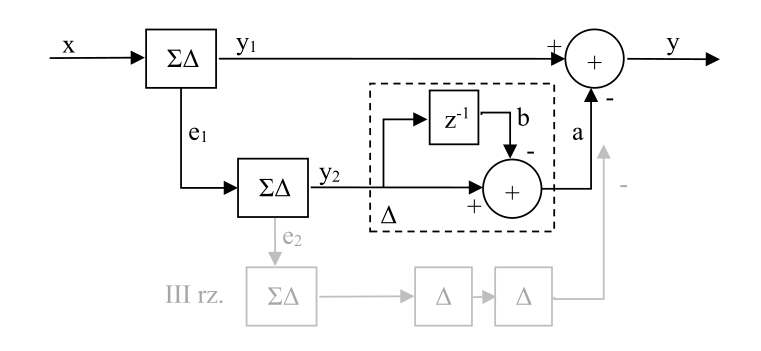
\includegraphics[width = \textwidth]{sigma_delta_II_III_order.png}
            \caption{Diagram przepływu sygnału w implementacji przetwornika Sigma-Delta drugiego i trzeciego  rzędu}
	\end{center}
\end{figure}
\section{Zagadnienia implementacyjne}
\subsection{Definicje badanych sygnałów}
Każda zaimplementowana instancja wzmacniacza klasy D będzie miała podany na wejście delikatnie zaszumiony sygnał sinusoidalny, by 
zasymulować rzeczywistą sytuację, kiedy to sygnał wejściowy również jest w pewnym stoniu zaszumiony. 
\[
\text{s[n]} = \frac{\sigma}{\sqrt{2}} \cdot \left( \text{randn}(\text{n}) + j \cdot \text{randn}(\text{n}) \right)
\]

\[
x_{pure}[n] = A \cdot e^{j \cdot \left( 2 \pi f_{n0} n + \phi_0 \right)}
\]
\[
    x_{in} = x_{pure}[n] + s[n]
\] gdzie
\\
s[n] - matematyczny zapis funkcji generującej szum biały, \\
$\sigma$ - odchylenie standardowe szumu \\
$x_{pure}[n]$ - czysty sygnał sinusoidalny, niezaszumiony \\
A - amplituda sygnału sinusoidalnego \\
$f_n$ - częstotliowść unormowana sygnału niezaszumionego \\
n - badana liczba próbek \\
$\phi_0$ - faza początkowa czystego sygnału
$x_{in}$ - sygnał podawany na wejście w każdej instancji badanego wzmacniacza klasy D \\

Sygnał odniesienia dla komparatora może być zdefiniowany jako sygnał rampowy \(x_{odn}[n]\), dany równaniem:
\[
x_{odn}[n] = 
\begin{cases} 
    0, & \text{dla } n < 0, \\
    k \cdot n, & \text{dla } n \geq 0,
\end{cases}
\]
gdzie \(k\) to współczynnik nachylenia rampy. \\

Schematy przepływu sygnału w stopniach wejściowych (obrazy 3, 5, 6) pokazują dokładnie, jak będzie wyglądał 
kod w matlabie implementujący ich konkretne funkcjonalności.
\subsection{Realizacja środkowego bloku wzmacniacza klasy D}
Ze względu na bardzo teoretyczny stopnień realizacji projektu, nie będzie implementowany 
"prawdziwy" stopnień pośrendni wzmacniacza klasy D, czyli wmacniacza napięcia, po którym sygnał trafia na układ wtórnika 
komplementarnego, ponieważ cały ten blok realizuje jedną funkcję - czyli wzmocnienie amplitudy sygnału. Skupimy się 
tutaj tylko na tym aspekcie, idealiując w pewnym sensie ten blok. Dla każdej instancji wzmacniacza klasy D blok ten 
będzie przyjmował sygnał i zwracał ten sygnał o zwiększonej amplitudzie. \\

\subsection{Dobór filtra}

Zaznaczone zostało, że sygnał, który będzie przetwarzany przez układ to sygnał audio - więc filtr, który 
będzie stopniem wyjściowym dla każdego układu będzie dobrany w iteracyjny sposób, by dla każdej realizacji ulepszał odtwarzanie 
sygnału z jego wersji cyfrowej. Ograniczenia filtru na chwilę obecną są bardzo luźno zdefiniowane:
\\
- rodzaj filtru: SOI, pasmowo - przepustowy; \\
- typ filtru: Butterwortha \\
- pasmo przepustowe: 20 Hz - 25kHz; \\


\end{document}